\documentclass[journal,12pt,twocolumn]{IEEEtran}

\usepackage{setspace}
\usepackage{gensymb}

\singlespacing


\usepackage[cmex10]{amsmath}

\usepackage{amsthm}

\usepackage{mathrsfs}
\usepackage{txfonts}
\usepackage{stfloats}
\usepackage{bm}
\usepackage{cite}
\usepackage{cases}
\usepackage{subfig}

\usepackage{longtable}
\usepackage{multirow}

\usepackage{enumitem}
\usepackage{mathtools}
\usepackage{steinmetz}
\usepackage{tikz}
\usepackage{circuitikz}
\usepackage{verbatim}
\usepackage{tfrupee}
\usepackage[breaklinks=true]{hyperref}

\usepackage{tkz-euclide}

\usetikzlibrary{calc,math}
\usepackage{listings}
    \usepackage{color}                                            %%
    \usepackage{array}                                            %%
    \usepackage{longtable}                                        %%
    \usepackage{calc}                                             %%
    \usepackage{multirow}                                         %%
    \usepackage{hhline}                                           %%
    \usepackage{ifthen}                                           %%
    \usepackage{lscape}     
\usepackage{multicol}
\usepackage{chngcntr}

\DeclareMathOperator*{\Res}{Res}

\renewcommand\thesection{\arabic{section}}
\renewcommand\thesubsection{\thesection.\arabic{subsection}}
\renewcommand\thesubsubsection{\thesubsection.\arabic{subsubsection}}

\renewcommand\thesectiondis{\arabic{section}}
\renewcommand\thesubsectiondis{\thesectiondis.\arabic{subsection}}
\renewcommand\thesubsubsectiondis{\thesubsectiondis.\arabic{subsubsection}}


\hyphenation{op-tical net-works semi-conduc-tor}
\def\inputGnumericTable{}                                 %%

\lstset{
%language=C,
frame=single, 
breaklines=true,
columns=fullflexible
}
\begin{document}


\newtheorem{theorem}{Theorem}[section]
\newtheorem{problem}{Problem}
\newtheorem{proposition}{Proposition}[section]
\newtheorem{lemma}{Lemma}[section]
\newtheorem{corollary}[theorem]{Corollary}
\newtheorem{example}{Example}[section]
\newtheorem{definition}[problem]{Definition}

\newcommand{\BEQA}{\begin{eqnarray}}
\newcommand{\EEQA}{\end{eqnarray}}
\newcommand{\define}{\stackrel{\triangle}{=}}
\bibliographystyle{IEEEtran}

\providecommand{\mbf}{\mathbf}
\providecommand{\pr}[1]{\ensuremath{\Pr\left(#1\right)}}
\providecommand{\qfunc}[1]{\ensuremath{Q\left(#1\right)}}
\providecommand{\sbrak}[1]{\ensuremath{{}\left[#1\right]}}
\providecommand{\lsbrak}[1]{\ensuremath{{}\left[#1\right.}}
\providecommand{\rsbrak}[1]{\ensuremath{{}\left.#1\right]}}
\providecommand{\brak}[1]{\ensuremath{\left(#1\right)}}
\providecommand{\lbrak}[1]{\ensuremath{\left(#1\right.}}
\providecommand{\rbrak}[1]{\ensuremath{\left.#1\right)}}
\providecommand{\cbrak}[1]{\ensuremath{\left\{#1\right\}}}
\providecommand{\lcbrak}[1]{\ensuremath{\left\{#1\right.}}
\providecommand{\rcbrak}[1]{\ensuremath{\left.#1\right\}}}
\theoremstyle{remark}
\newtheorem{rem}{Remark}
\newcommand{\sgn}{\mathop{\mathrm{sgn}}}
\providecommand{\abs}[1]{\left\vert#1\right\vert}
\providecommand{\res}[1]{\Res\displaylimits_{#1}} 
\providecommand{\norm}[1]{\left\lVert#1\right\rVert}
%\providecommand{\norm}[1]{\lVert#1\rVert}
\providecommand{\mtx}[1]{\mathbf{#1}}
\providecommand{\mean}[1]{E\left[ #1 \right]}
\providecommand{\fourier}{\overset{\mathcal{F}}{ \rightleftharpoons}}
%\providecommand{\hilbert}{\overset{\mathcal{H}}{ \rightleftharpoons}}
\providecommand{\system}{\overset{\mathcal{H}}{ \longleftrightarrow}}
	%\newcommand{\solution}[2]{\textbf{Solution:}{#1}}
\newcommand{\solution}{\noindent \textbf{Solution: }}
\newcommand{\cosec}{\,\text{cosec}\,}
\providecommand{\dec}[2]{\ensuremath{\overset{#1}{\underset{#2}{\gtrless}}}}
\newcommand{\myvec}[1]{\ensuremath{\begin{pmatrix}#1\end{pmatrix}}}
\newcommand{\mydet}[1]{\ensuremath{\begin{vmatrix}#1\end{vmatrix}}}

\numberwithin{equation}{subsection}

\makeatletter
\@addtoreset{figure}{problem}
\makeatother
\let\StandardTheFigure\thefigure
\let\vec\mathbf

\renewcommand{\thefigure}{\theproblem}

\def\putbox#1#2#3{\makebox[0in][l]{\makebox[#1][l]{}\raisebox{\baselineskip}[0in][0in]{\raisebox{#2}[0in][0in]{#3}}}}
     \def\rightbox#1{\makebox[0in][r]{#1}}
     \def\centbox#1{\makebox[0in]{#1}}
     \def\topbox#1{\raisebox{-\baselineskip}[0in][0in]{#1}}
     \def\midbox#1{\raisebox{-0.5\baselineskip}[0in][0in]{#1}}
\vspace{3cm}
\title{Assignment 7}
\author{Sri Harsha CH}

\maketitle
\newpage

\bigskip
\renewcommand{\thefigure}{\theenumi}
\renewcommand{\thetable}{\theenumi}

\begin{abstract}
This document explains the method of finding the equation of circle.
\end{abstract}

Download all python codes from 
\begin{lstlisting}
https://github.com/harshachinta/EE5609-Matrix-Theory/tree/master/Assignments/Assignment7/code
\end{lstlisting}
%
and latex-tikz codes from 
%
\begin{lstlisting}
https://github.com/harshachinta/EE5609-Matrix-Theory/tree/master/Assignments/Assignment7
\end{lstlisting}
%
\section{Problem}
Find the equation of the circle passing through $\myvec{0\\0}$ and making intercepts a and b on the coordinate axes.
\section{Explanation}
The equation of a circle can be expressed as,
\begin{align}
    \vec{x}^{T}\vec{x} - 2\vec{c}^{T}\vec{x} +f=0 \label{eq:eq1}
\end{align}
where $\vec{c}$ is the center.\\
Given the circle makes intercepts a and b on the coordinate axis. Let intercept on x-axis be a and the intercept on y-axis be b.\\
Therefore the points are,
\begin{align}
    \vec{P_1}=\myvec{0\\0} \quad \vec{P_2}=\myvec{a\\0} \quad \vec{P_3}=\myvec{0\\b} \label{eq:eq2}
\end{align}
Substituting $\vec{P_1}$ from equation \eqref{eq:eq2} in \eqref{eq:eq1} we get,
\begin{align}
    &\myvec{0&0}\myvec{0\\0} -2\myvec{c1&c2}\myvec{0\\0}+f=0\\
    &\implies \boxed{f=0} \label{eq:eq3}
\end{align}
Substituting $\vec{P_2}$ from equation \eqref{eq:eq2} in \eqref{eq:eq1} we get,
\begin{align}
    &\myvec{a&0}\myvec{a\\0} -2\myvec{c1&c2}\myvec{a\\0}+0=0\\
    &a^{2}-2(ac_1)=0\\
    &\implies \boxed{c_1=\frac{a}{2}} \label{eq:eq4}
\end{align}
Substituting $\vec{P_3}$ from equation \eqref{eq:eq2} in \eqref{eq:eq1} we get,
\begin{align}
    &\myvec{0&b}\myvec{0\\b} -2\myvec{c1&c2}\myvec{0\\b}+0=0\\
    &b^{2}-2(bc_2)=0\\
    &\implies \boxed{c_2=\frac{b}{2}} \label{eq:eq5}
\end{align}
\renewcommand{\thefigure}{\arabic{figure}}
\begin{figure}[h!]
	\centering
	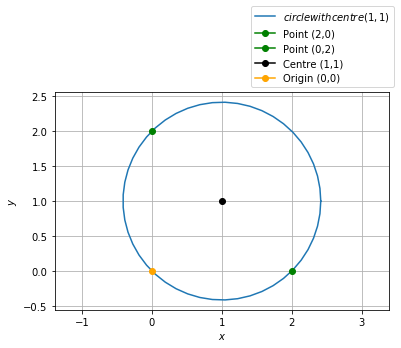
\includegraphics[width=\columnwidth]{circle.png}
	\caption{Circle passing through origin and making intercept on coordinate axes}
	\label{myfig}
\end{figure}\\
\\
Thus, from equation \eqref{eq:eq4} and \eqref{eq:eq5},\\ The center of circle is,
\begin{align}
    \implies \boxed{\vec{c} = \myvec{c_1\\c_2} = \frac{1}{2}\myvec{a\\ b}}
\end{align}
The radius of the circle is,
\begin{align}
    r=\sqrt{\vec{c}^{T}\vec{c}-f}\\
\implies \boxed{r=\sqrt{\frac{a^2+b^2}{4}}} \label{eq:eq6}
\end{align}

Therefore,\\ The equation of circle is,
\begin{align}
    \implies \boxed{\vec{x}^{T}\vec{x} - \myvec{a&b}\vec{x}=0} \label{eq:eq7}
\end{align}
\section{Solution}
The equation of circle is,
\begin{align}
    \boxed{\vec{x}^{T}\vec{x} - \myvec{a&b}\vec{x}=0} \label{eq:eq1}
\end{align}
\\\end{document}
